\chapter{Régression Linéaire et Sélection de Modèles}
\section{Informations Générales du Cours}
\begin{itemize}
    \item \textbf{Structure :} Alternance entre cours magistraux et travaux pratiques (lab sessions) en R ou Python.
    \item \textbf{Contact :} fabien.navarro@univ-paris1.fr.
    \item \textbf{Évaluation :} Un examen final de 2h (le 13/03), sans session de rattrapage.
    \item \textbf{Ouvrages de référence :} \textit{The Elements of Statistical Learning} (ESL, Hastie et al., 2009)  et \textit{An Introduction to Statistical Learning} (ISL, James et al., 2021/23).
\end{itemize}

\section{Introduction et Problématique}
\begin{itemize}
    \item L'objectif central de la régression est d'expliquer une quantité (la variable à expliquer, $Y$) par d'autres variables (les variables explicatives ou prédicteurs, $X$).
    \item Les objectifs peuvent être descriptifs, c'est-à-dire comprendre comment les prédicteurs affectent la quantité à expliquer.
    \item Ils peuvent également être prédictifs, ce qui consiste à prédire la quantité à expliquer en connaissant les prédicteurs.
    \item On parle de "régression" lorsque la variable $Y$ est quantitative , et de "classification" ou "discrimination" lorsqu'elle est qualitative.

\begin{figure}[h]
    \centering
    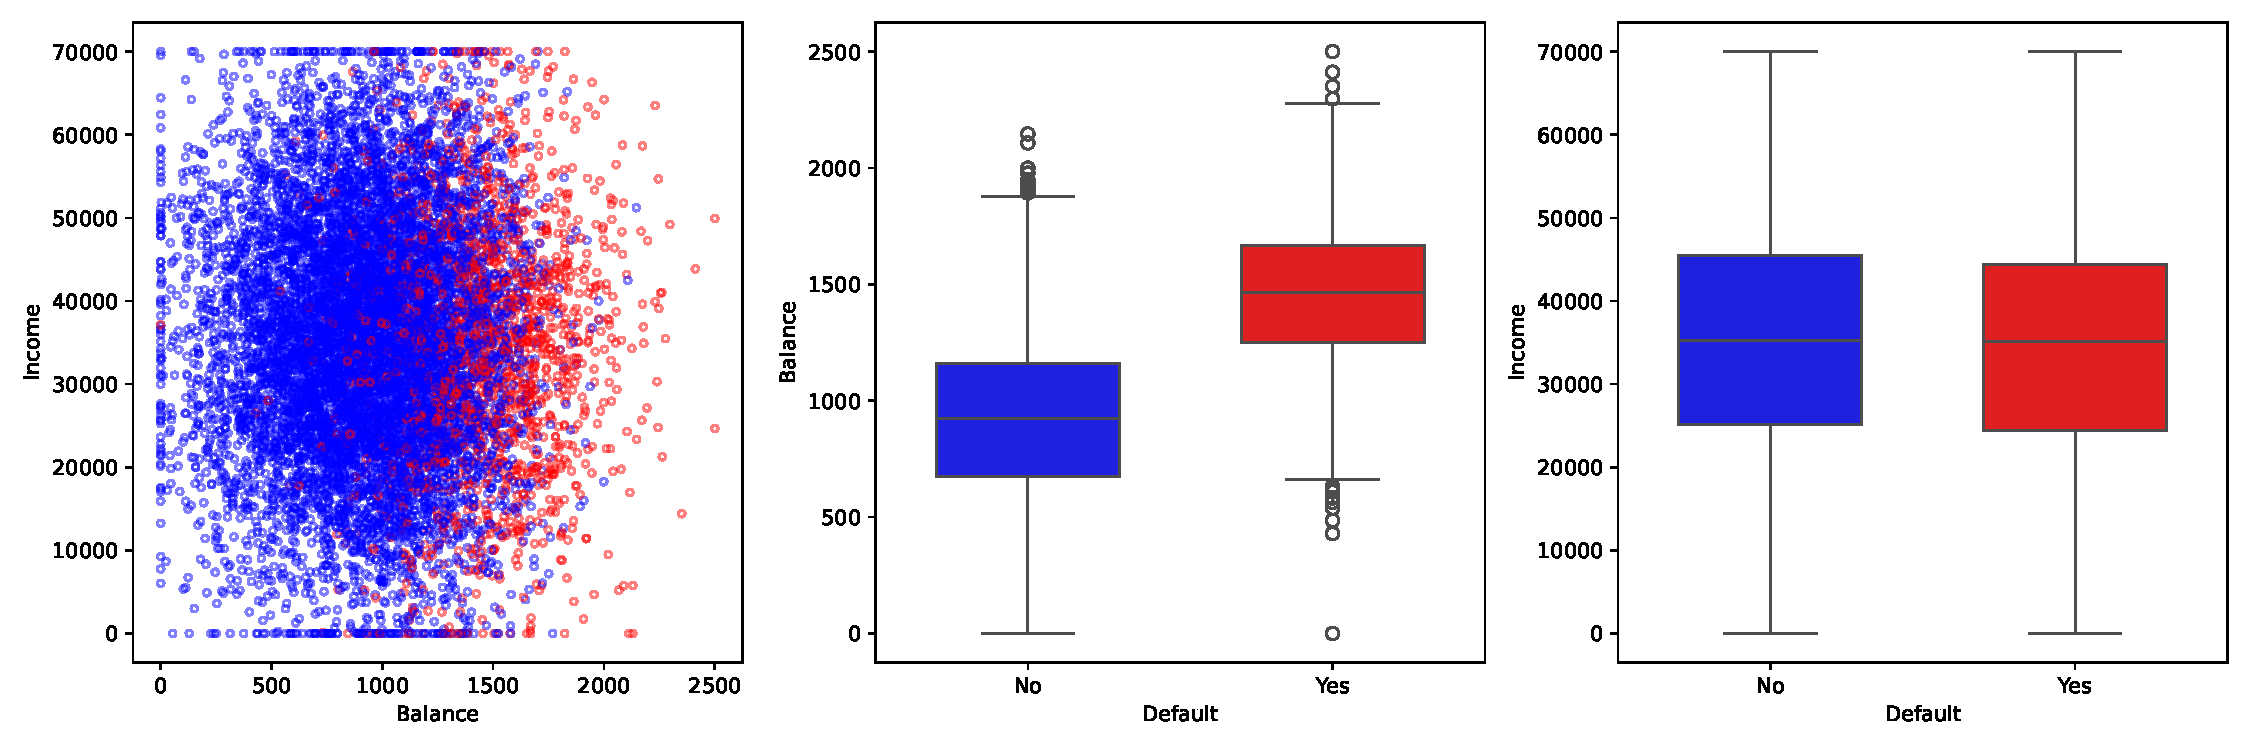
\includegraphics[width=\textwidth]{images/default_data.pdf}
    \caption{Exemple de tâche de classification (Prédire le Default de paiement en fonction du solde et des revenus)}
    \label{fig:default_data}
\end{figure}

\begin{figure}[h]
    \centering
    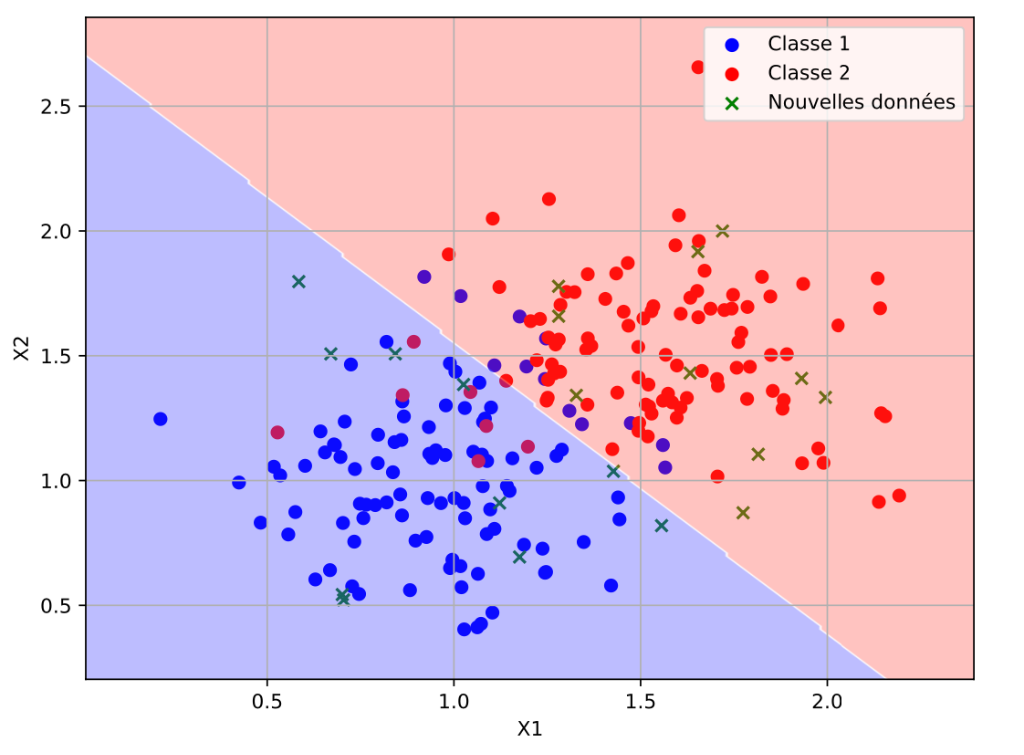
\includegraphics[width=0.7\textwidth]{images/decision_boundary.png}
    \caption{Illustration d'une frontière de décision pour un problème de classification binaire}
    \label{fig:decision_boundary}
\end{figure}

    \item Le modèle général se formule par $Y = f(X) + \epsilon$ , où $f$ est une fonction inconnue de $X$ et $\epsilon$ un terme d'erreur indépendant de $X$. Le but est d'estimer $f$ à partir des observations.
    \item Le modèle linéaire suppose que $f$ est une fonction linéaire : $f(X) = \beta_0 + \beta_1 X_1 + \dots + \beta_p X_p$. L'estimation de $f$ est grandement simplifiée puisqu'il suffit d'estimer $p+1$ coefficients au lieu d'une fonction en $p$ dimensions.
    \item Bien que les relations réelles soient rarement strictement linéaires, la régression linéaire reste extrêmement utile sur les plans conceptuel et pratique. Elle offre de nets avantages en matière d'interprétabilité et de performances prédictives (faible biais si la relation réelle est quasi-linéaire).
    \item Cependant, si le nombre d'observations $n$ est proche de $p$ ($n \ge p$), le modèle peut souffrir de surapprentissage (overfitting) et d'une forte variance. Si $n < p$, la méthode des moindres carrés classique est inopérante : la matrice $X^T X$ n'est pas inversible (il y a plus d'inconnues que d'équations), le système admet une infinité de solutions et l'estimateur n'est plus unique (ce que l'on traduit parfois par un "sur-paramétrage" ou une variance infinie).
    \item Pour améliorer les modèles linéaires, on peut utiliser la sélection de sous-ensembles (Subset Selection) , les méthodes de pénalisation/régularisation (Shrinkage comme Ridge ou Lasso) pour réduire la variance , ou la réduction de dimension.
\end{itemize}

\begin{figure}[h]
    \centering
    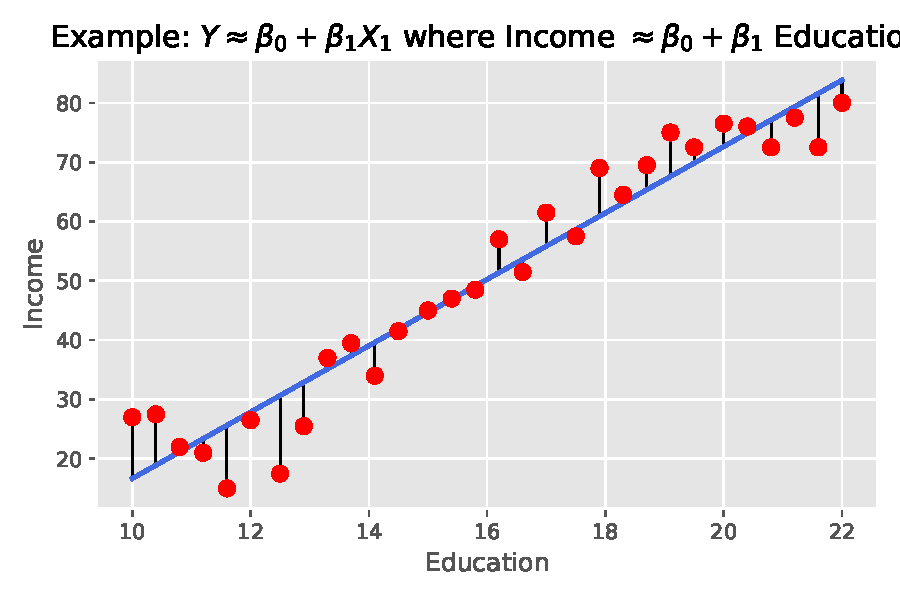
\includegraphics[width=0.6\textwidth]{images/income_lm.pdf}
    \caption{Exemple de relation quasi-linéaire ($Income \approx \beta_0 + \beta_1 Education$)}
    \label{fig:income_lm}
\end{figure}

\begin{figure}[h]
    \centering
    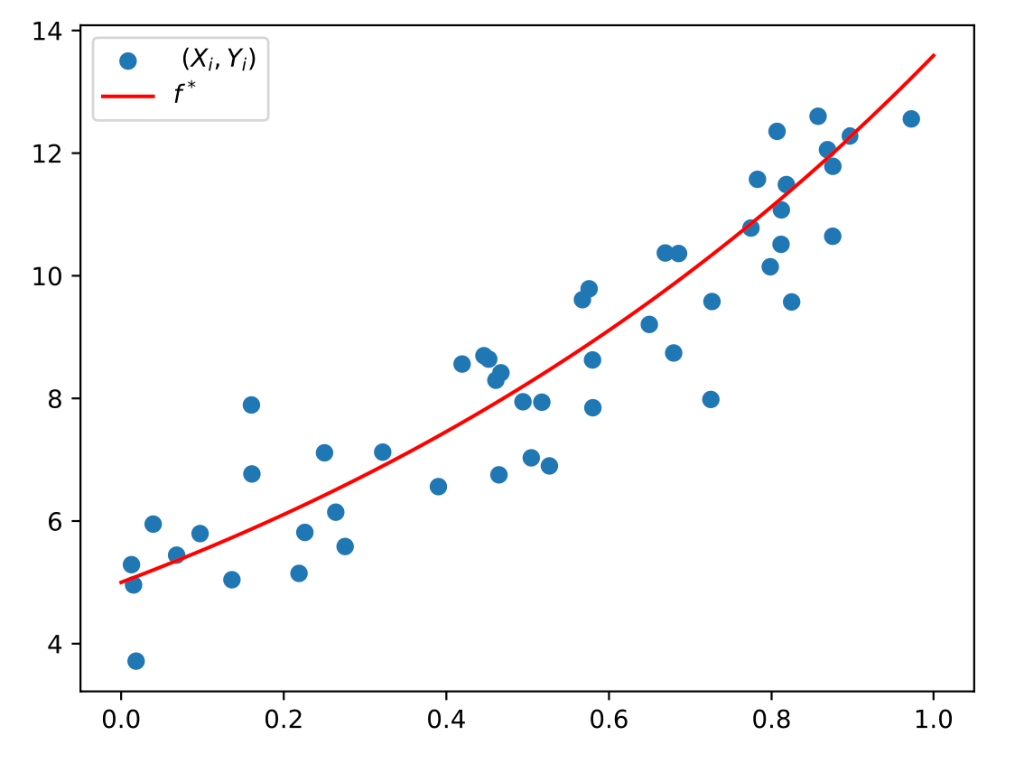
\includegraphics[width=0.7\textwidth]{images/regression_fit.png}
    \caption{Ajustement d'un modèle de régression linéaire simple sur un nuage de points}
    \label{fig:regression_fit}
\end{figure}

\section{Modèles Linéaires (Multiple Linear Regression)}
\subsection{Définition et Modélisation}
\begin{itemize}
    \item Les données se composent de $n$ observations $(Y, X_1, \dots, X_p)$ notées $(y_i, x_{1,i}, \dots, x_{p,i})$.
    \item L'équation du modèle linéaire multiple (mlm) postule l'existence de $p+1$ paramètres inconnus tels que $Y_i = \beta_0 + \beta_1 x_{1,i} + \dots + \beta_p x_{p,i} + \epsilon_i$.
    \item Sous forme matricielle, le modèle s'écrit $Y = X\beta + \epsilon$. Ici, $Y \in \mathbb{R}^n$ est le vecteur des réponses, $X \in \mathbb{R}^{n \times (p+1)}$ est la matrice de design, $\beta \in \mathbb{R}^{p+1}$ est le vecteur des coefficients, et $\epsilon \in \mathbb{R}^n$ est le terme d'erreur.
    \item On suppose que la variance des erreurs est constante : $Var(\epsilon_i) = \sigma^2$. Le modèle est qualifié de gaussien si $\epsilon_i \sim \mathcal{N}(0, \sigma^2)$.
\end{itemize}

\begin{figure}[h]
    \centering
    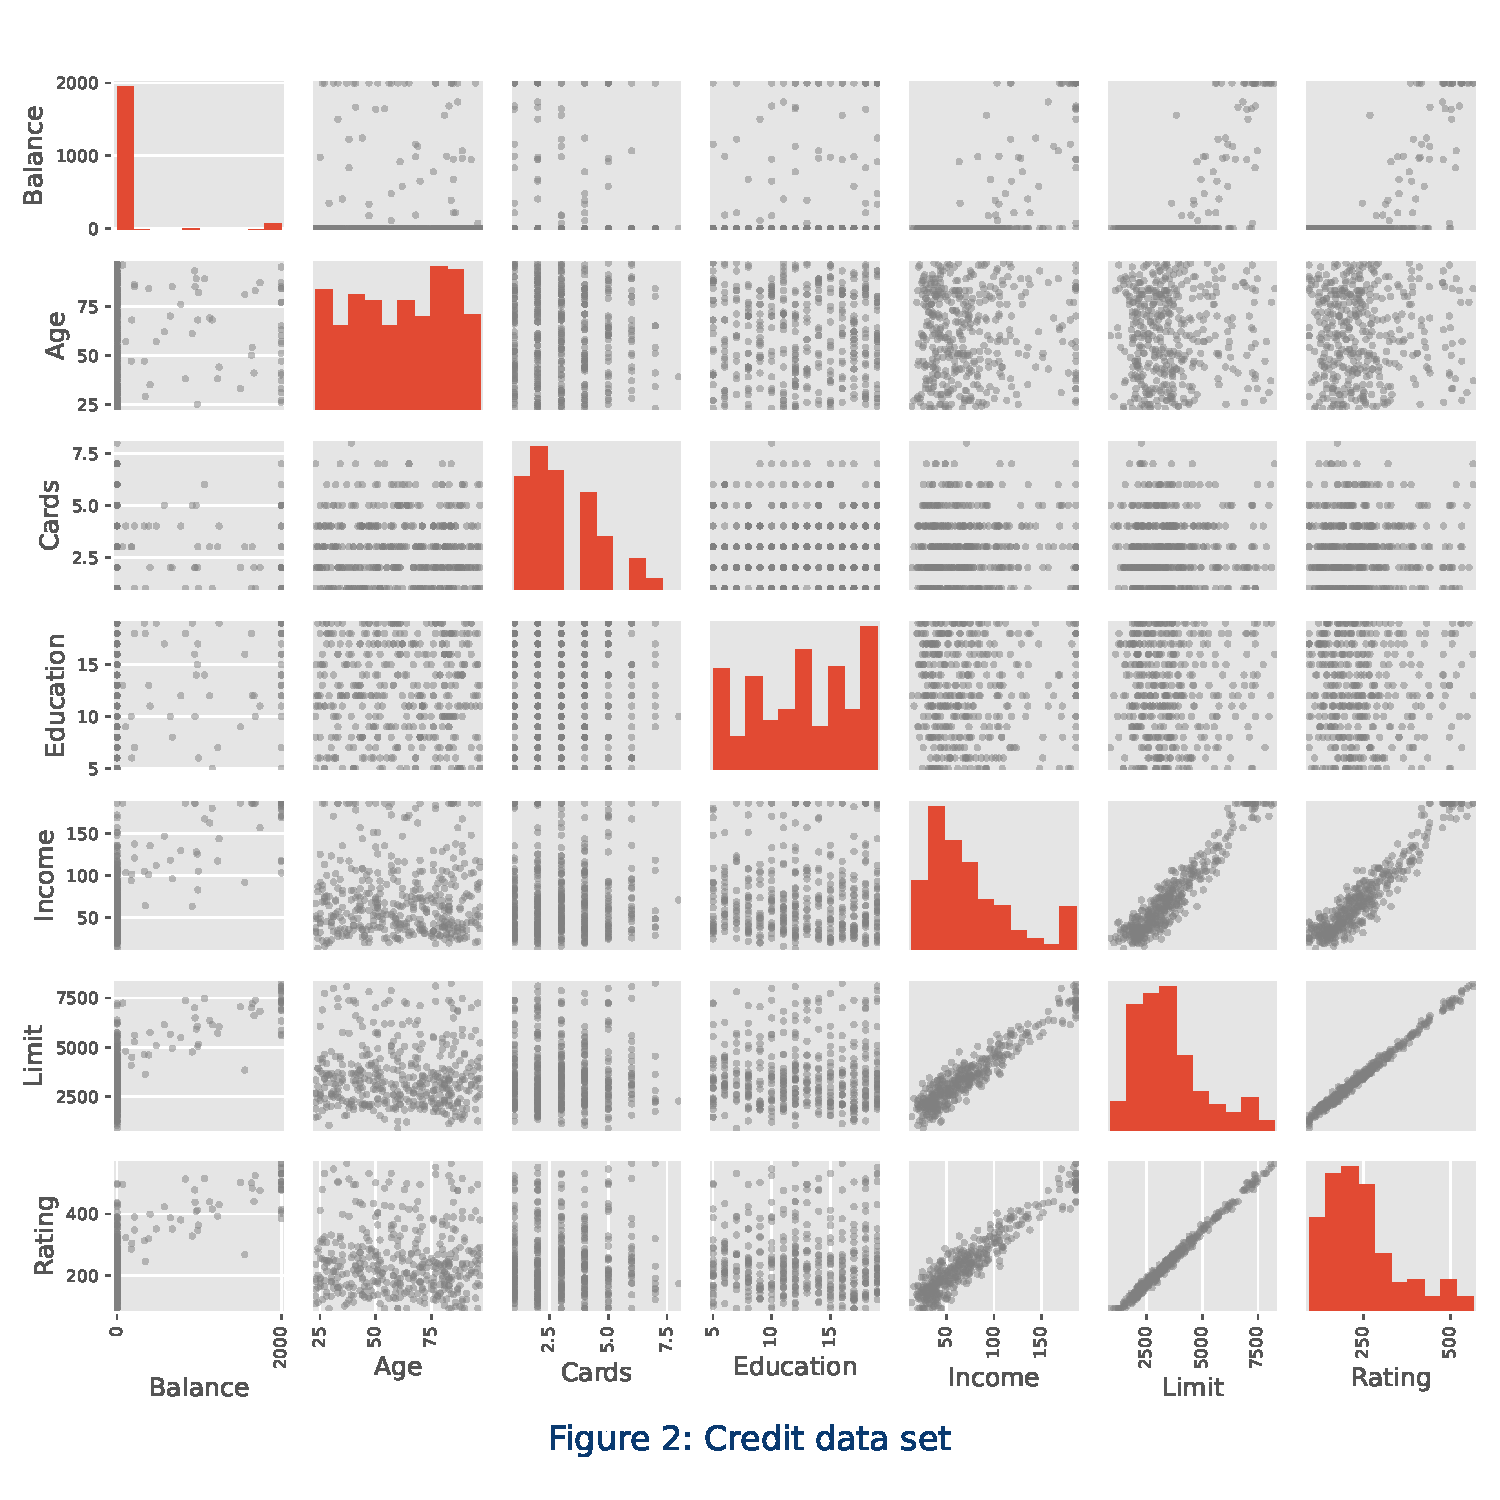
\includegraphics[width=0.8\textwidth]{images/credit_pairs.pdf}
    \caption{Matrice de nuages de points (Scatterplot Matrix) pour le dataset Credit}
    \label{fig:credit_pairs}
\end{figure}

\subsection{Estimation par Moindres Carrés Ordinaires (OLS)}
\begin{itemize}
    \item L'estimateur OLS est construit pour minimiser l'erreur d'estimation : $\hat{\beta} = \arg\min_{\beta \in \mathbb{R}^{p+1}} ||Y - X\beta||^2$.
    \item Il correspond à la solution des équations normales : $X^T X \beta - X^T Y = 0$.
    \item L'estimation des paramètres est donnée par la formule $\hat{\beta} = (X^T X)^{-1} X^T Y$.
    \item Les valeurs ajustées (prédites) sont $\hat{Y} = X\hat{\beta} = H Y$, où $H = X(X^T X)^{-1} X^T$ est appelée la matrice "chapeau" (hat matrix).
    \item Le vecteur des résidus est calculé par $e = Y - \hat{Y} = (I - H)Y$.
    \item Selon le théorème de Gauss-Markov, les estimateurs OLS sont dits "BLUE" (Best Linear Unbiased Estimators) : ils sont sans biais et de variance minimale parmi les estimateurs linéaires sans biais.
\end{itemize}

\subsection{Évaluation du Modèle}
\begin{itemize}
    \item La somme des carrés des résidus est définie par $RSS = \sum_{i=1}^n e_i^2 = \sum_{i=1}^n (y_i - \hat{y}_i)^2$.
    \item L'écart-type résiduel (RSE) estime l'écart-type de l'erreur $\sigma$ et se calcule par $\hat{\sigma} = RSE = \sqrt{\frac{RSS}{n-2}}$ (dans le cas simple).
    \item La qualité d'ajustement est aussi mesurée par le $R^2$, représentant la fraction de variance expliquée : $R^2 = 1 - \frac{RSS}{TSS}$, où le $TSS$ (Total Sum of Squares) est $\sum_{i=1}^n (y_i - \bar{y})^2$. Plus le $R^2$ est grand, plus le modèle explique efficacement la variance des données.
\end{itemize}

\section{Sélection de Sous-ensembles (Subset Selection)}

Afin de pallier la complexité d'un modèle incluant de multiples variables non pertinentes (ce qui nuit à l'interprétabilité), plusieurs techniques de sélection existent.

\subsection{Best Subset Selection}
\begin{itemize}
    \item Soit $\mathcal{M}_0$ le modèle nul, qui ne contient aucun prédicteur et prédit systématiquement la moyenne de l'échantillon.
    \item Pour $k=1, 2, \dots, p$, on ajuste la totalité des $\binom{p}{k}$ modèles contenant très exactement $k$ prédicteurs. \textbf{($\bigstar$ EXAMEN)} Au total, cela demande d'ajuster $2^p$ modèles, un calcul qui explose rapidement en complexité.
    \item Parmi ces modèles de taille $k$, on retient le meilleur (celui ayant le plus petit RSS ou le plus grand $R^2$), que l'on nomme $\mathcal{M}_k$. \textbf{($\bigstar$ EXAMEN) Attention au piège de l'emboîtement :} le modèle $\mathcal{M}_k$ n'est absolument pas garanti de contenir les variables du modèle $\mathcal{M}_{k-1}$. Les modèles successifs dans "Best Subset" ne sont donc généralement pas emboîtés.
    \item Enfin, on choisit un unique modèle optimal parmi la séquence $\mathcal{M}_0, \dots, \mathcal{M}_p$ en se basant sur des critères pénalisés comme le $C_p$ (AIC), le BIC, le $R^2$ ajusté, ou l'erreur de validation croisée.
\end{itemize}

\begin{figure}[h]
    \centering
    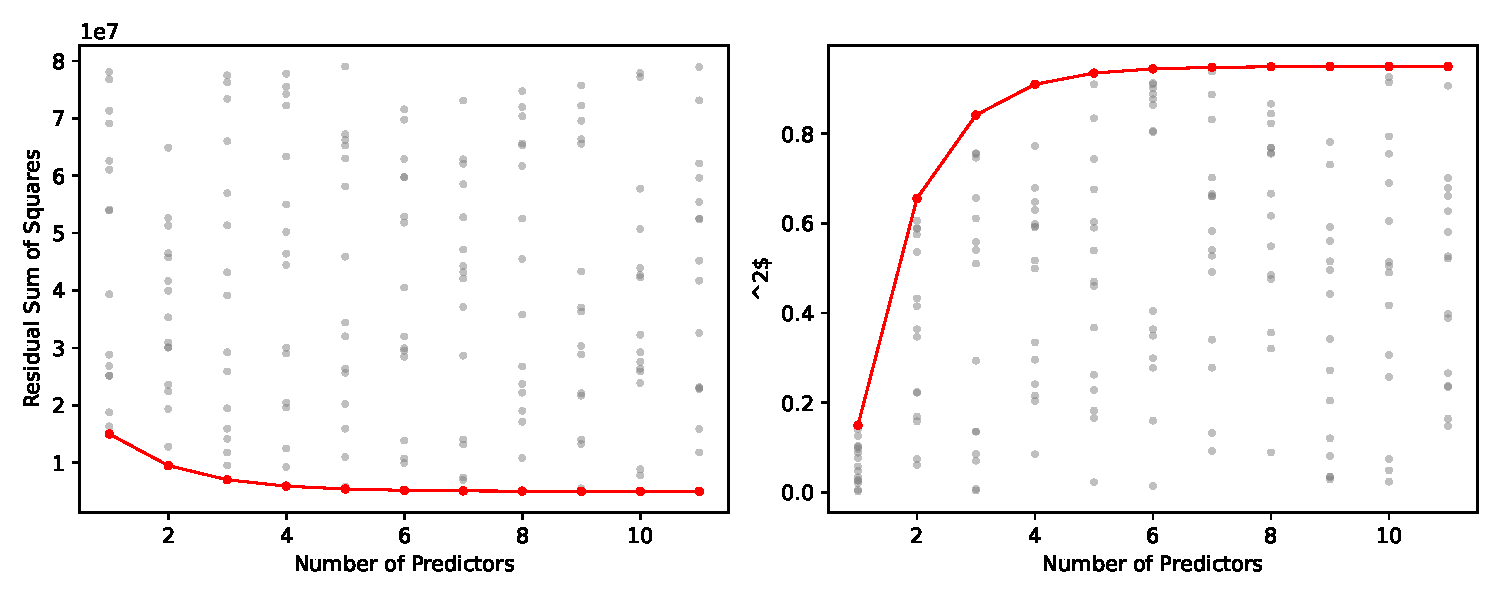
\includegraphics[width=\textwidth]{images/subset_selection.pdf}
    \caption{RSS et $R^2$ pour l'ensemble des modèles ajustés en fonction du nombre de prédicteurs. La courbe rouge relie les meilleurs modèles $\mathcal{M}_k$.}
    \label{fig:subset_rss_r2}
\end{figure}

\subsection{Traitement des Variables Qualitatives (Dummy Variables)}
\begin{itemize}
    \item Si un prédicteur qualitatif possède deux niveaux (ex: genre), on crée une variable indicatrice valant 1 ou 0. Le choix de la valeur (ex: 0 pour homme, 1 pour femme) est arbitraire et n'altère pas l'ajustement global, mais il change l'interprétation des coefficients.
    \item Si le prédicteur possède plus de deux niveaux, une seule variable indicatrice ne suffit pas. On crée alors de multiples variables indicatrices, au nombre de niveaux moins un.
    \item Le niveau ne disposant pas de variable indicatrice propre est utilisé comme catégorie de référence (baseline).
\end{itemize}

\subsection{Stepwise Selection (Méthodes Pas-à-Pas)}
La sélection "Best Subset" devient trop onéreuse en calcul lorsque $p$ est grand (nécessité de calculer $2^p$ modèles) et risque d'engendrer un surapprentissage (overfitting). Les méthodes Stepwise offrent une alternative plus rapide.

SUB\section*{Forward Stepwise Selection}
\begin{itemize}
    \item Commence par le modèle nul $\mathcal{M}_0$.
    \item À chaque itération $k$ (de $0$ à $p-1$), l'algorithme évalue les $p-k$ modèles qui ajoutent un unique prédicteur supplémentaire au modèle $\mathcal{M}_k$. \textbf{($\bigstar$ EXAMEN) Propriété clé :} Étant donné qu'on ne fait qu'ajouter, les modèles sont \textbf{emboîtés}. Les variables du modèle $\mathcal{M}_k$ sont un sous-ensemble strict des variables du modèle $\mathcal{M}_{k+1}$.
    \item Le meilleur de ces $p-k$ modèles (plus petit RSS ou plus grand $R^2$) est sélectionné et nommé $\mathcal{M}_{k+1}$.
    \item \textbf{($\bigstar$ EXAMEN) Avantage computationnel :} cette approche n'ajuste qu'environ $1 + p(p+1)/2$ modèles au total, contre $2^p$ pour Best Subset. Elle peut s'appliquer même dans le cas critique où $n < p$.
    \item Inconvénient : il n'y a aucune garantie que le modèle sélectionné soit le meilleur possible parmi tous les $2^p$ modèles existants.
\end{itemize}

SUB\section*{Backward Stepwise Selection}
\begin{itemize}
    \item Commence à l'inverse, par le modèle complet $\mathcal{M}_p$ contenant tous les prédicteurs.
    \item À chaque itération $k$ (de $p$ à $1$), on évalue les $k$ modèles formés en retirant exactement un prédicteur de $\mathcal{M}_k$. Comme pour le Forward, ces modèles sont \textbf{emboîtés} (les variables de $\mathcal{M}_{k-1}$ sont un sous-ensemble de $\mathcal{M}_k$). \textbf{($\bigstar$ EXAMEN)} La complexité de calcul est aussi de l'ordre de $1 + p(p+1)/2$ modèles.
    \item Le meilleur est retenu comme $\mathcal{M}_{k-1}$.
    \item Contrainte forte : exige impérativement que $n > p$ afin de pouvoir ajuster le modèle complet initial.
\end{itemize}

\subsection{Critères de Choix du Modèle Optimal}
Le RSS et le $R^2$ calculés sur les données d'entraînement diminuent mécaniquement à mesure que le nombre de variables augmente, ce qui les rend inaptes pour sélectionner la bonne taille de modèle. Il faut recourir à d'autres indicateurs pour estimer l'erreur de test (soit indirectement via pénalité, soit directement).

\begin{itemize}
    \item \textbf{$C_p$ de Mallows / AIC :} Estime l'erreur de test via $C_p = \frac{1}{n} (RSS + 2 d \hat{\sigma}^2)$, où $d$ est la dimension du modèle. Dans le cadre d'erreurs gaussiennes, l'AIC ($-2 \log L + 2d$) est équivalent au $C_p$.
    \item \textbf{BIC :} Se calcule par $BIC = \frac{1}{n} (RSS + \log(n) d \hat{\sigma}^2)$. Il remplace le facteur $2$ de l'AIC par $\log(n)$. \textbf{($\bigstar$ EXAMEN) Point crucial :} puisque $\log(n) > 2$ pour $n > 7$, le BIC pénalise plus lourdement la complexité que l'AIC. En conséquence, le BIC a tendance à sélectionner des modèles plus petits (plus parcimonieux) que l'AIC.
    \item \textbf{$R^2$ Ajusté :} Défini par $1 - \frac{RSS / (n - d - 1)}{TSS / (n - 1)}$. Contrairement au $R^2$ usuel, il pénalise l'inclusion de variables superflues.
    \item \textbf{Validation Croisée (CV) et Validation Set :} L'erreur de test est estimée directement (sans estimer $\sigma^2$ ni $d$) en retirant une partie des données. 
    \begin{itemize}
        \item \textbf{Attention cruciale de Leakage :} la sélection des variables doit impérativement s'effectuer \textit{uniquement} sur le jeu d'entraînement pour chaque sous-échantillon. Faire la sélection sur l'ensemble complet avant la CV introduirait un biais majeur sous-estimant fortement l'erreur réelle.
        \item \textbf{($\bigstar$ EXAMEN) Ré-Ajustement Final (Refit sur données complètes) :} Une fois que la taille ou le sous-ensemble optimal de variables a été choisi par validation (par exemple "le modèle contenant les variables 1, 3, 5 et 8 est le meilleur"), il est **impératif de réajuster l'équation finale sur l'intégralité du dataset disponible (Train + Validation)**. Le *validation set* ne sert qu'à sélectionner les *dimensions* ou le sous-ensemble ; le modèle livré in fine doit bénéficier de l'estimation de coefficients ($\beta$) la plus précise possible, usant de la totalité des données existantes.
    \end{itemize}
\end{itemize}

\begin{figure}[h]
    \centering
    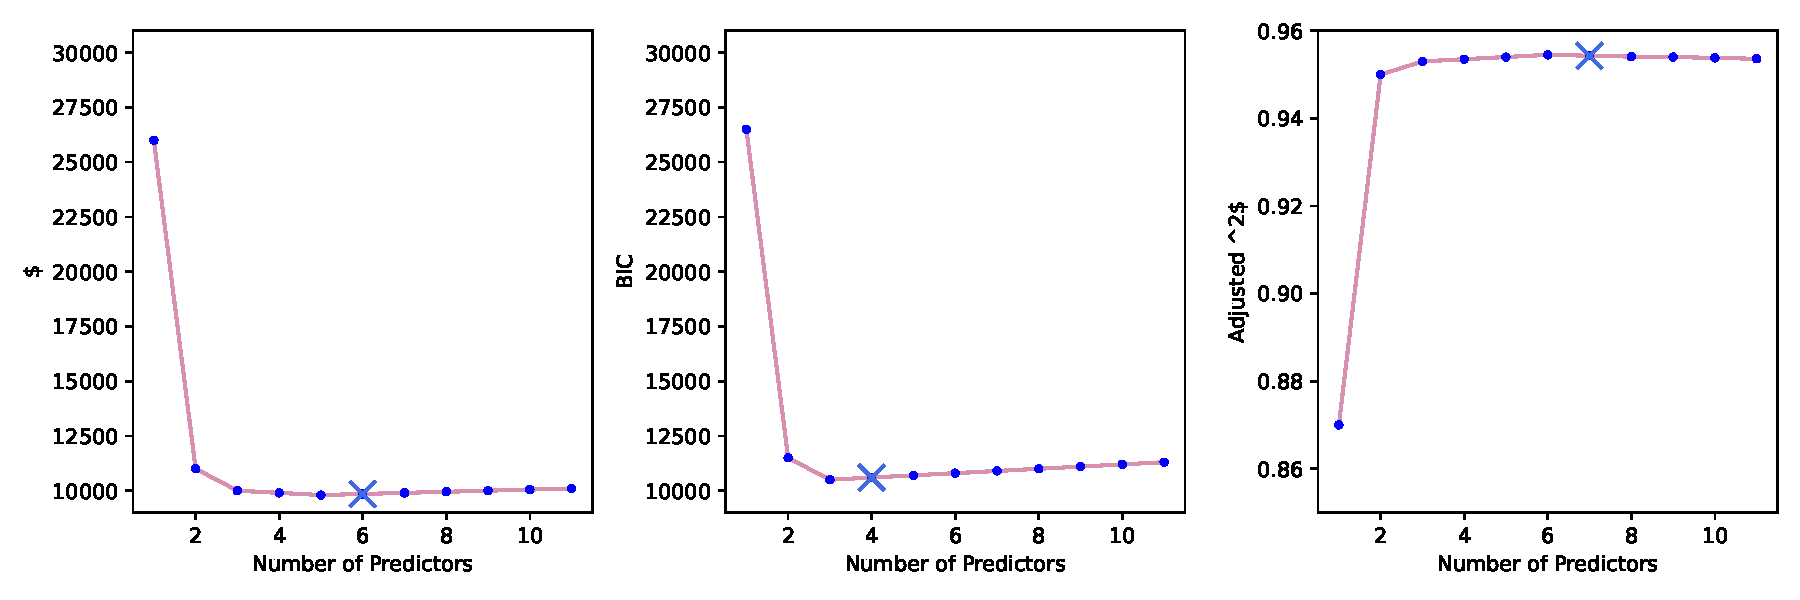
\includegraphics[width=0.9\textwidth]{images/subset_cp_bic_adjr2.pdf}
    \caption{Critères de sélection pénalisés ($C_p$, BIC, $R^2$ ajusté) appliqués à la séquence de modèles $\mathcal{M}_k$.}
    \label{fig:subset_criteria}
\end{figure}

\section{Implémentation Pratique en R (Extraits)}
\begin{itemize}
    \item Importer des données : \texttt{read.table("fichier.txt", header=T)} ou \texttt{read.csv()}.
    \item Supprimer une colonne (ex: index) : \texttt{Credit[,"X"] <- NULL}.
    \item Inspecter la structure des données : \texttt{str(Credit)}. Visualiser les corrélations : \texttt{ggpairs()}.

\begin{figure}[h]
    \centering
    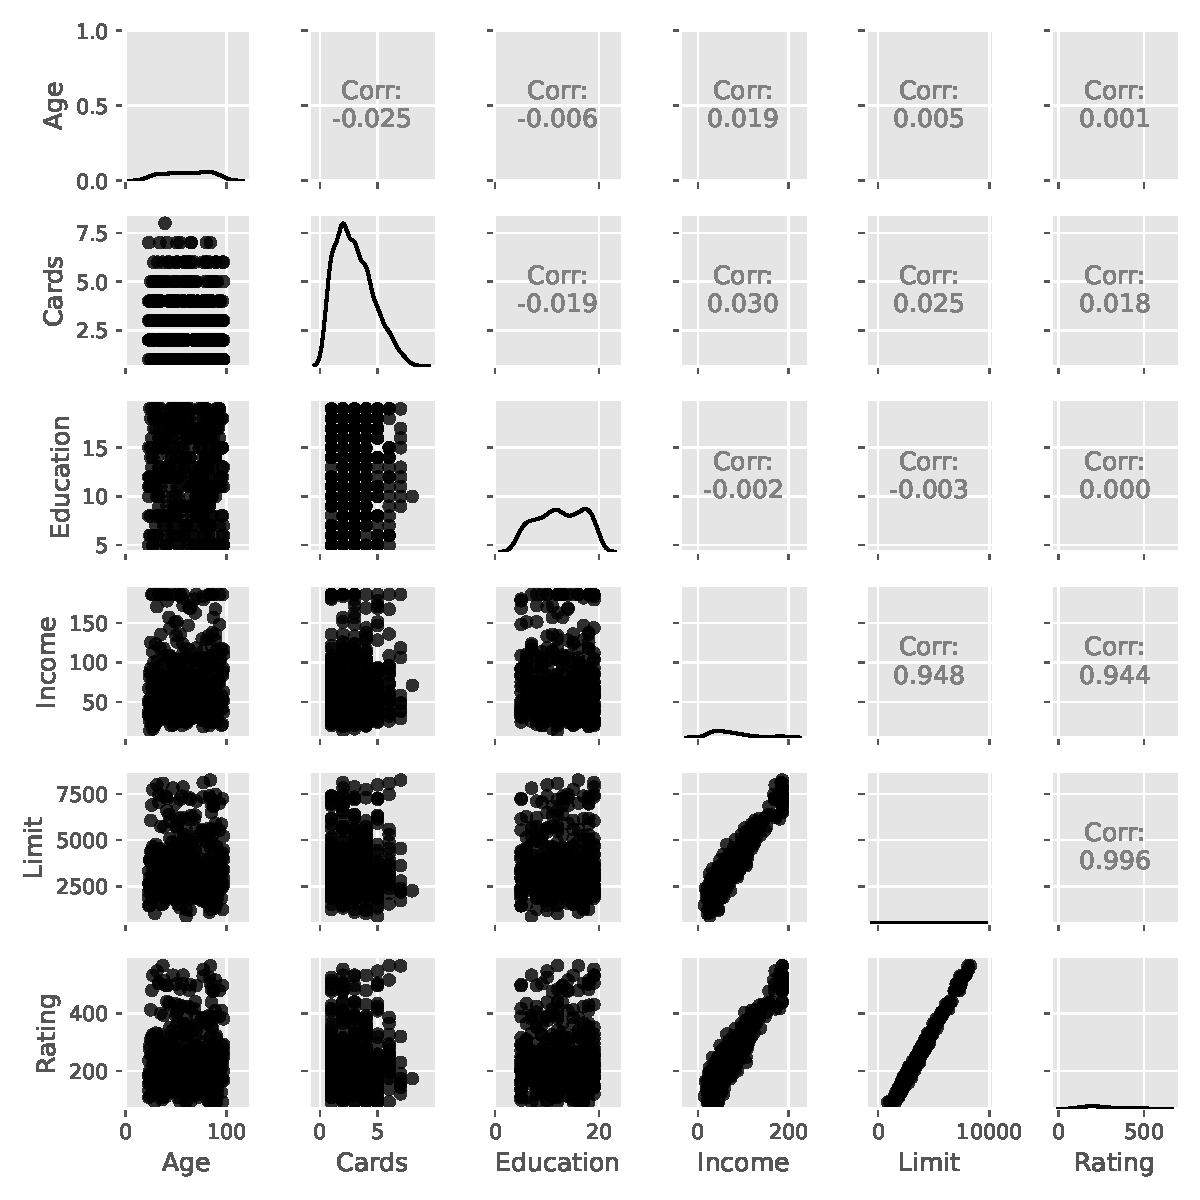
\includegraphics[width=0.6\textwidth]{images/credit_ggpairs.pdf}
    \caption{Visualisation avancée avec \texttt{ggpairs} (corrélations et densités)}
    \label{fig:credit_ggpairs}
\end{figure}

    \item Ajuster un modèle linéaire : \texttt{reg <- lm(Y \textasciitilde{} X1, data=w)}. Résumé statistique complet : \texttt{summary(reg)}.
    \item Prédire une nouvelle valeur : \texttt{predict(reg, data.frame(X1=8), interval="confidence")}.
    \item Intervalles de confiance des coefficients : \texttt{confint(reg, level=0.95)}.
    \item Best Subset Selection : utiliser la librairie \texttt{leaps} avec \texttt{regsubsets(Balance \textasciitilde{} ., data=Credit, nvmax=11)}.
    \item Forward Selection : ajouter l'argument \texttt{method="forward"} dans \texttt{regsubsets}.
    \item Scinder les données en Test/Train aléatoirement : \texttt{train <- sample(c(TRUE,FALSE), nrow(Credit), rep=TRUE)}. \textit{Attention : cette méthode assigne chaque ligne au train ou au test avec 50\% de chance, la taille finale varie donc. Pour forcer une proportion exacte (ex: 80\% / 20\%), on utilisera plutôt \texttt{train <- sample(1:nrow(Credit), size = floor(0.8*nrow(Credit)))}}.
    \item Créer une matrice de design pour gérer automatiquement les \textit{dummy variables} sur les données de test : \texttt{model.matrix(Balance \textasciitilde{} ., data=Credit[test,])}. \textbf{Important :} C'est impératif pour s'assurer que les indicatrices de test sont construites de manière identique au train, évitant un décalage si un niveau catégoriel manque dans le jeu de test.
\end{itemize}
